\documentclass[11pt,english]{article}

\setlength\parindent{0pt}
\usepackage{amssymb,amsmath,amscd,graphicx,fontenc,bbold,bm,amsthm,mathrsfs,mathtools}

\usepackage{algorithm, algorithmic}

% code and psendocode
\usepackage{verbatim}
\usepackage{minted}
\usemintedstyle{trac}

% colors
\usepackage{xcolor}
\definecolor{LightGray}{gray}{0.95}
\definecolor{DarkGray}{gray}{0}

\usepackage{minted} % code listing
\usemintedstyle{trac}

\definecolor{LightGray}{gray}{0.95}

% new commands
\newcommand{\code}[1]{{\small\colorbox{LightGray}{\texttt{#1}}}}
\newcommand{\tr}{\mathrm{Trace}}
\newcommand{\real}{\mathbb{R}}
\newcommand{\sigmoid}{\mathrm{sigmoid}}
\newcommand{\softmax}{\mathrm{softmax}}
\newcommand{\sign}{\mathrm{sign}}
\newcommand{\abs}{\mathrm{abs}}
\newcommand{\rect}{\mathrm{rect}}
\newcommand{\onehot}{\mathrm{onehot}}
\newcommand{\relu}{\mathrm{relu}}
\newcommand{\pd}[1]{\frac{\partial}{\partial {#1}}}

\usepackage[top=3cm,bottom=3cm,right=2.3cm,left=2.3cm,twoside=false]{geometry}

\title{IFT6390-fundamentals of machine learning\\Assignment 3}
\author{Jonathan Guymont, Marzieh Mehdizadeh, Mohammad Bardestani}

\date{}

\begin{document}

\maketitle

\section*{Question 1}
(a) 
\begin{equation}
\begin{split}
0.5(\tanh(0.5x)+1) =& 0.5 (\frac{e^{0.5x}-e^{-0.5x}}{e^{0.5x}+e^{-0.5x}}+1)\\
=& 0.5 (\frac{1-e^{-x}}{1+e^{-x}}+\frac{1+e^{-x}}{1+e^{-x}})\\
=& 0.5\frac{2}{1+e^{-x}}\\
=& \frac{1}{1+e^{-x}}\\
\end{split}
\end{equation}

(b) 
\begin{equation}
\begin{split}
\log \sigmoid(x)=& \log (1+e^{-x})^{-1}\\
=& - \log (1+e^{-x})\\
=& -\softmax(-x)
\end{split}
\end{equation}

(c)

\begin{equation}
\begin{split}
\frac{d}{dx}\sigmoid(x) =& \frac{d}{dx} (1+e^{-x})^{-1}\\
=& -(1+e^{-x})^{-2}\frac{d}{dx} 1+e^{-x} \\
=& (1+e^{-x})^{-2}e^{-x}\\
=& (1+e^{-x})^{-1}\frac{e^{-x}}{1+e^{-x}}\\
=& (1+e^{-x})^{-1}(\frac{1+e^{-x}-1}{1+e^{-x}})\\
=& (1+e^{-x})^{-1}(1- \frac{1}{1+e^{-x}})\\
\end{split}
\end{equation}

(4) 
\begin{equation}
\begin{split}
\tanh'(x)=& (\frac{e^x-e^{-x}}{e^x+e^{-x}})'\\
=& \frac{(e^x+e^{-x})(e^x+e^{-x})-(e^x-e^{-x})(e^x-e^{-x})}{(e^x+e^{-x})^2}\\
=& \frac{(e^x+e^{-x})^2-(e^x-e^{-x})^2}{(e^x+e^{-x})^2}\\
=& 1- \frac{(e^x-e^{-x})^2}{(e^x+e^{-x})^2}\\
=& 1 - \tanh^2(x)
\end{split}
\end{equation}

(5) $\sign(x) = -1 + 2\cdot \mathbb{1}_{x>0}$ \\

(6) $\abs'(x)=\sign(x)$\\

(7) $\rect'(x) = \mathbb{1}_{x>0}$ \\

(8) Let $f(\bm{x})=\sum_{x_i \in \bm{x}} x_i^2$, then $f'(\bm{x})=(f'_{x_1},...,f'_{x_{|\bm{x}|}})=(2x_1,...,2x_{|\bm{x}|})$\\

(9) Let $f(\bm{x})=\sum_{x_i \in \bm{x}} |x_i|$, then $f'(\bm{x})=(f'_{x_1},...,f'_{x_{|\bm{x}|}})=(\sign(x_1),...,\sign(x_{|\bm{x}|}))$\\

\section*{Gradient Computation for Parameters optimizations in a neural net for multiclass classification}

(1) The dimension of $\bm{b}^{(1)}$ is $d_h \times 1$. The formula of the preactivation vector is 
\[
	\bm{h}^a = \bm{W}^{(1)}\bm{x} + \bm{b}^{(1)} 
\]
and the formula for obtaining the value of the element $j$ is
\[
	\bm{h}_j^a = \bm{W_{j,\cdot}}^{(1)}\bm{x} + \bm{b}_j^{(1)}
	=\bm{b}_j^{(1)} + \sum_{i=1}^d \bm{W_{j,i}}^{(1)}\bm{x}_i.
\]
The output vector of the activation is given by
\[
	\bm{h}^s = \relu(\bm{h}^a)
\]
where $\relu(\cdot)$ is applied element wise, i.e. $\bm{h}_j^s = \max(0, \bm{h}_j^a)$, $j=1,...,d_h$.\\

(2) The dimension of $\bm{W}^{(2)}$ is $m \times d_h$ and the dimension of $\bm{b}^{(2)}$ is $m \times 1$. 
\[
	\bm{o}^a = \bm{W}^{(2)}\bm{h}^s + \bm{b}^{(2)}
\]
\[
	\bm{o}_k^a 
	= \bm{W}_{k,\cdot}^{(2)}\bm{h}^s + \bm{b}_k^{(2)}
	= \bm{b}_k^{(2)} + \sum_{i=1}^{d_h} \bm{W_{k,i}}^{(2)}\bm{h}^s_i
\]
for $k=1,..,m$.\\

(3) 
\begin{equation}
	\bm{o}^s_k = \frac{\exp(\bm{o}_k^a)}{\sum_{k=1}^m \exp(\bm{o}_k^a)}
	\label{eq:softmax}
\end{equation}
They are all positive because $\exp\colon \real \mapsto \real^+$. Also a sum of positive number is positive. And the ratio of a posive number over a positive number is also positive.
\[
	\sum_{k=1}^m \bm{o}^s_k = \frac{1}{\sum_{k=1}^m \exp(\bm{o}_k^a)} \sum_{k=1}^m \exp(\bm{o}_k^a)=1  	
\]

(4) Let $Z=\sum_{k=1}^m \exp(\bm{o}_k^a)$. Then $\bm{o}^s=\frac{1}{Z}(\exp(\bm{o}_1^a),...,\exp(\bm{o}_m^a))^\top$ and 
\[
	L(\bm{x}, y) = -\log \onehot_m(y) (\exp(\bm{o}_1^a(\bm{x}))/Z,...,\exp(\bm{o}_m^a(\bm{x}))/Z)^\top
	= -\log \onehot_m(y)\bm{o}^s(\bm{x})
\]
where $\onehot_m(y)$ is a $1 \times  m$ onehot representation for $y$.\\
 
(5) $\hat{R}$ is an estimation of the expected value of the loss function (minus the loglikelihood in our case)
\[
	\hat{R} = \frac{1}{n}\sum_{i=1}^n L(x^{(i)}, y^{(i)})=\frac{1}{n}\sum_{i=1}^n 
	-\log \onehot_m(y^{(i)})\bm{o}^s(\bm{x}^{(i)})
\]
The set of trainable parameters is $\bm{\theta}=\{W^{(1)}, W^{(2)}, b^{(1)}, b^{(2)}\}$. The number of scalar parameters is $n_\theta=d_h\cdot d + d_h + m\cdot d_h + m=d_h(d+1)+m(d_h+1)$. \\

\textbf{Optimization problem.} First we need to initialize the parameters properly. To find the parameters that minimize the loss, we need to compute the derivative of the loss function w.r.t each parameters. Then we update each parameters by moving them in the opposite direction of their gradient (since we minimize). We repeat this step until a stopping criterion is met (e.g. maximum number of iteration is reached when using early stopping).\\

(6)
\begin{algorithm}[H]
	\begin{algorithmic}
		\REQUIRE Step size $\eta$
		\REQUIRE Initial parameter $\bm{\omega}_0$
		\REQUIRE Number of iterations $T$
		\FOR{$i=1$ to $T$}
		\STATE Compute gradient $\bm{g}_t=\frac{1}{m}\nabla_{\bm{\omega}}\sum_i L(\bm{x}^{(i)}, \bm{y}^{(i)})$ 
		\STATE Apply update: $\bm{\omega}_t=\bm{\omega}_{t-1}-\eta \bm{g}_t$
		\ENDFOR
	\end{algorithmic}
	\caption{Pseudocode for Batch Gradient Descent}
	\label{alg:seq}
\end{algorithm}

(7) 

\begin{equation}
\begin{split}
	\pd{\bm{o}^a}L
	=& \pd{\bm{o}^a} -\log \onehot_m(y)\bm{o}^s\\
	=& -\frac{1}{\onehot_m(y)\bm{o}^s}\pd{\bm{o}^a} \onehot_m(y)\bm{o}^s \\
	=& -\frac{1}{\onehot_m(y)\bm{o}^s}\pd{\bm{o}^a} \onehot_m(y)\softmax(\bm{o}^a) \\ 
	=& -\frac{1}{\onehot_m(y)\bm{o}^s}\onehot_m(y) \softmax(\bm{o}^a)(\onehot_m(y)-\softmax(\bm{o}^a)) \\
	=& - (\onehot_m(y)-\softmax(\bm{o}^a))
\end{split}
\end{equation}

(8) 

\begin{minted}[bgcolor=LightGray, fontsize=\footnotesize]{python}
onehot = np.zeros(m)
onehot[y] = 1
grad_oa = os - onehot
\end{minted}

(9) From the previous exercise we have 
$$
\frac{\partial L}{\partial\bm{o}^a}=\bm{o}^s-\onehot_m(y).
$$
and so
\begin{equation}\label{oka}
\frac{\partial L}{\partial o_i^a}=o_i^s-{\onehot_m(y)}_i,
\end{equation}
where ${\onehot_m(y)}_i$ is the $i$'th component of $\onehot_m(y)$. 
From~\eqref{ok} we deduce that
$$
\frac{\partial o_i^a}{\partial W_{kj}^{(2)}}=
\begin{cases}
h_j^s &  i=k;\\
0 & \text{otherwise}. 
\end{cases}
$$
Moreover from~\eqref{ok}
\begin{equation}
\frac{\partial o_i^a}{\partial b_k^{(2)}}=\begin{cases}
1 & i=k;\\
0 & \text{otherwise}.
\end{cases}
\end{equation}
Putting these together we obtain 
\begin{equation}
\begin{split}
\frac{\partial L}{\partial W_{kj}^{(2)}}&=\sum_{i=1}^m\frac{\partial L}{\partial o_i^a}\frac{\partial o_i^a}{\partial W_{kj}^{(2)}}=\left(o_k^s-\onehot_m(y)_k\right)h_j^{s}\\[.2cm]
\frac{\partial L}{\partial b_k^{(2)}}&=\sum_{i=1}^m\frac{\partial L}{\partial {o_i}^a}\frac{\partial o_i}{\partial b_k^{(2)}}=o_k^s-\onehot_m(y)_k.
\end{split}
\end{equation} 

(10) Since $\frac{\partial\bm{o}^a}{\partial\bm{W}^{(2)}}=\bm{h}^{s}$ and $\frac{\partial L}{\partial\bm{o}^a}=\bm{o}^s-\onehot_m(y)$, then 
\begin{equation}
\frac{\partial L}{\partial\bm{W}^{(2)}}=\frac{\partial L}{\partial\bm{o}^a}\cdot\frac{\partial\bm{o}^a}{\partial\bm{W}^{(2)}}=(\bm{o}^s-\onehot_y(y))\bm{h}^{s}.
\end{equation}
Moreover, since $\frac{\partial\bm{o}^a}{\partial\bm{b}^{(2)}}=\bm{1}$, we obtain
\begin{equation}
\frac{\partial L}{\partial\bm{b}^{(2)}}=\frac{\partial L}{\partial\bm{o}^a}\cdot\frac{\partial\bm{o}^a}{\partial\bm{b}^{2}}=\bm{o}^s-\onehot_m(y).
\end{equation}
We remark that $\bm{W}^{2}\in\mathbb{R}^{d_h\times m}$, $\bm{b}^{(2)}\in\mathbb{R}^m$, $\bm{o}^a\in \mathbb{R}^m$, $\bm{h}^s\in \mathbb{R}^{d_h}$ and $\frac{\partial L}{\partial\bm{o}^a}\in\mathbb{R}^m$.

\begin{minted}[bgcolor=LightGray, fontsize=\footnotesize]{python}
grad_b_2 = grad_oa
grad_W_2 = grad_ha.dot(X)
\end{minted}

(11) From~\eqref{ok} we see that
$$
\frac{\partial o_k^a}{\partial h_j^s}=W_{kj}^{(2)}.
$$
From~\eqref{oka} we deduce that
$$
\frac{\partial L}{\partial h_j^s}=\sum_{k=1}^m \left(o_k^s-\onehot_m(y)_k\right)w_{kj}^{(2)}.
$$
We recall that $o_k^s-\onehot_m(y)_k$ is the $k$'th component of the vector $\bm{o}^s-\onehot_m(y)$

(12)
$$
\nabla L=(\bm{o}^s-\onehot_m(y))\bm{W}^{(2)\top}.
$$

\begin{minted}[bgcolor=LightGray, fontsize=\footnotesize]{python}
grad_hs = grad_oa.T.dot(self.W_2)
\end{minted}

(13) We jest need to emphasis that
\begin{equation}\label{char}
\frac{\partial h_j^s}{\partial h_j^a}=
\begin{cases}
0 & h_j^a<0;\\
1 & h_j^a>0.
\end{cases}
\end{equation}
Note that $\frac{\partial h_j^s}{\partial h_j^a}$ is not defined $h_j^a=0$.

(14) We have 
$$
\frac{\partial L}{\partial\bm{h}^a}=\frac{\partial L}{\partial\bm{h}^s}\frac{\partial \bm{h}^s}{\partial \bm{h}^a}.
$$
where the components of $\frac{\partial \bm{h}^s}{\partial\bm{h}^a}$ is computes as in~\eqref{char}.

\bigskip
{\noindent\color{red} Part 15}
From the chain rule we have 
$$
\frac{\partial L}{\partial W_{kj}^{(1)}}=\sum_{i=1}^{d_h}\frac{\partial L}{\partial h_i^a}\frac{\partial h_i^a}{\partial W_{kj}^{(1)}}.
$$
Since 
$$
\bm{h}^a=\bm{W}^{(1)\top}\bm{x}+\bm{b}^{(1)},
$$
we get 
$$
\frac{\partial h_i^a}{\partial W_{kj}^{(1)}}=x_k. 
$$
For $\bm{b}^{(1)}$, from the chain rule we obtain 
$$
\frac{\partial L}{\partial b_{j}^{(1)}}=\sum_{i=1}^{d_h}\frac{\partial L}{\partial h_i^a}\frac{\partial h_i^a}{\partial b_{j}^{(1)}}.
$$
But 
$$
\frac{\partial h_i^a}{\partial b_{j}^{(1)}}=1.
$$

(16)
$$
\frac{\partial L}{\partial \bm{W}^{(1)}}=\frac{\partial L}{\partial \bm{h}^a}\bm{x}
$$
and 
$$
\frac{\partial L}{\partial \bm{b}^{1}}=\bm{1}.
$$

(17)
$$
\frac{\partial L}{\partial\bm{x}}=\frac{\partial L}{\partial\bm{h}^a}\frac{\partial \bm{h}^a}{\partial\bm{x}}.
$$
But 
$$
\frac{\partial \bm{h}^a}{\partial\bm{x}}=\bm{W}^\top.
$$

(18)
The gradient $L_1$ and $L_2$ regularization in term of two parameters $\bm{W}^{(1)}$ and $\bm{W}^{(2)}$ is a follows:

\begin{equation}
\begin{split}
\nabla_{\bm{W^{(1)}}}(L)= \lambda_{11}   \sign(\bm{W^{(1)}})+ 2\lambda_{12} {\bm{W}}^{(1)}
\end{split}
\end{equation}

\begin{equation}
\begin{split}
\nabla_{\bm{W^{(2)}}}(L)= \lambda_{21}   \sign(\bm{W^{(2)}})+ 2 \lambda_{22} {\bm{W}}^{(2)}
\end{split}
\end{equation}

where the sign is the matrix of sing of components of each $\bm{W^{(1)}}$ and $\bm{W^{(2)}}$. 

$$
\bm{W}^{(1)} \leftarrow \bm{W}^{(1)}- \eta \left( \nabla_{\bm{W^{(1)}}}\mathcal{R} + \nabla_{\bm{W^{(1)}}}\mathcal{L}\right)
$$
$$
\bm{W}^{(2)} \leftarrow \bm{W}^{(2)}- \eta \left( \nabla_{\bm{W^{(2)}}}\mathcal{R} + \nabla_{\bm{W^{(2)}}}\mathcal{L}\right)
$$


\textbf{Question 3: Practical part}\\

\begin{table}[h!]
	\centering
	\begin{tabular}{|c|c|}
		\hline 
		Loop backward & Matrix calculus backward \\ 
		\hline 
		$\sim$40 sec. & $\sim$5 sec. \\ 
		\hline 
	\end{tabular} 
	\caption{Training time on the cicles dataset. The training set represent 70\% if the data. The hidden layer size was set to 10, the learning rate was 0.05, the batch size was 32, the number of epoch was 1000.}
\end{table}

\newpage

\textbf{6. For loop to matrix calculus}

\begin{minted}[bgcolor=LightGray, fontsize=\footnotesize]{python}
def backward(self, X, Y):
    """Backward probagation
    
    Loop implementation. Afer each iteration the gradient 
    of the current example is added to the batch gradient.
    the gradient is divided by the size of the batch.
    
    Args
        X: (array) input batch of dimension <k x d>
        Y: (array) target batch of dimension <k x 1>
    """
    for x, y in zip(X, Y):
        # x as shape <1 x d>
        # y is int (y is change to onehot in self._onehot())
        self.forward(x, train=True)
        grad_oa    = self.os - self._onehot(y).T
        grad_hs    = grad_oa.T.dot(self.W_hy)
        grad_hs_ha = self._relu_prime(self.ha)       
        grad_ha    = grad_hs_ha * grad_hs.T          

        self.grad_W_hy  += grad_oa.dot(self.hs.T) / batch_size
        self.grad_b_hy  += grad_oa.reshape(grad_oa.shape[0], 1) / batch_size 
        self.grad_W_xh  += grad_ha.dot(x) / batch_size                
        self.grad_b_xh  += grad_ha.reshape(grad_ha.shape[0], 1) / batch_size
\end{minted}

\begin{minted}[bgcolor=LightGray, fontsize=\footnotesize]{python}
def backward(self, X, Y):
    """Backward probagation (without loop)

    Args
        X: (array) input batch of dimension <k x d>
        Y: (array) target batch of dimension <k x 1>
    """

    self.forward(X, train=True)
    grad_oa    = self.os - self._onehot(Y).T
    grad_hs    = grad_oa.T.dot(self.W_hy)
    grad_hs_ha = self._relu_prime(self.ha)       
    grad_ha    = grad_hs_ha * grad_hs.T          
    
    self.grad_W_hy  = grad_oa.dot(self.hs.T) / batch_size      
    self.grad_b_hy  = np.sum(grad_oa, axis=1).reshape(grad_oa.shape[0], 1) / batch_size
    self.grad_W_xh  = grad_ha.dot(X) / batch_size               
    self.grad_b_xh  = np.sum(grad_ha, axis=1).reshape(grad_ha.shape[0], 1) / batch_size
\end{minted}

\begin{figure}
	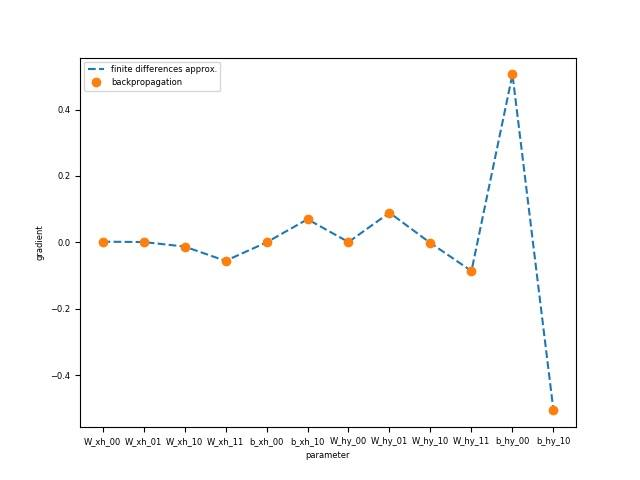
\includegraphics[width=\linewidth]{pic4.jpg}
	\caption{Question 2: Gradients for one example.}
	\label{fig:boat1}
\end{figure}

\begin{figure}
	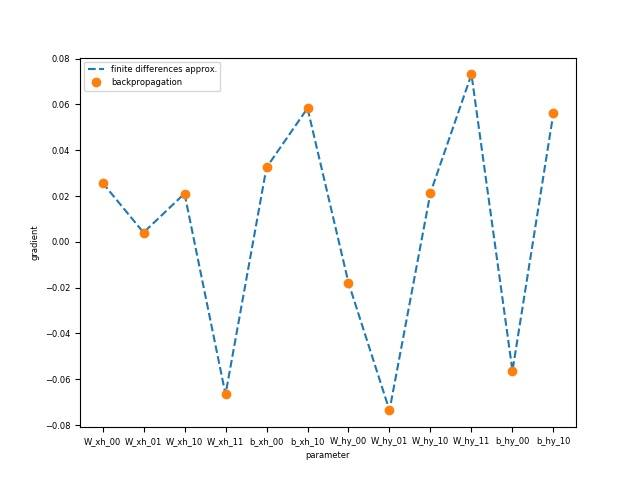
\includegraphics[width=\linewidth]{pic3.jpg}
	\caption{Question 4: Gradients for 10 example.}
	\label{fig:boat1}
\end{figure}

\begin{figure}
	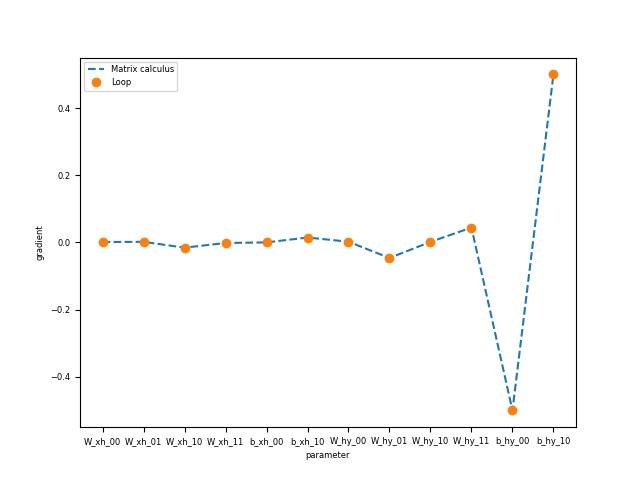
\includegraphics[width=\linewidth]{pic2.jpg}
	\caption{Question 7 a): Gradients for a batch of size 1.}
	\label{fig:boat1}
\end{figure}

\begin{figure}
	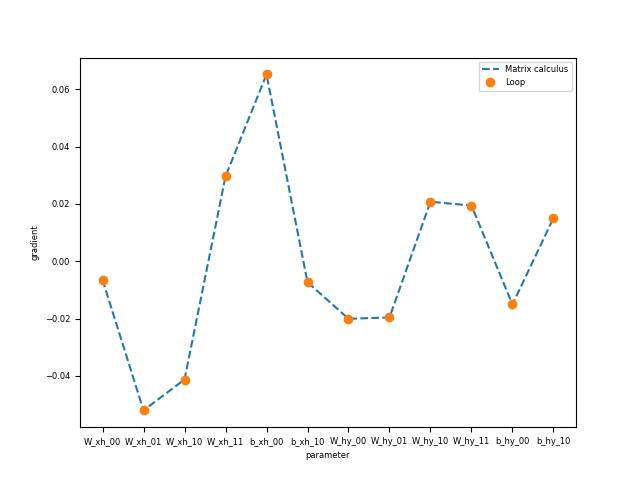
\includegraphics[width=\linewidth]{pic1.jpg}
	\caption{Question 7 b): Gradients for 10 example.}
	\label{fig:boat1}
\end{figure}

\begin{figure}
	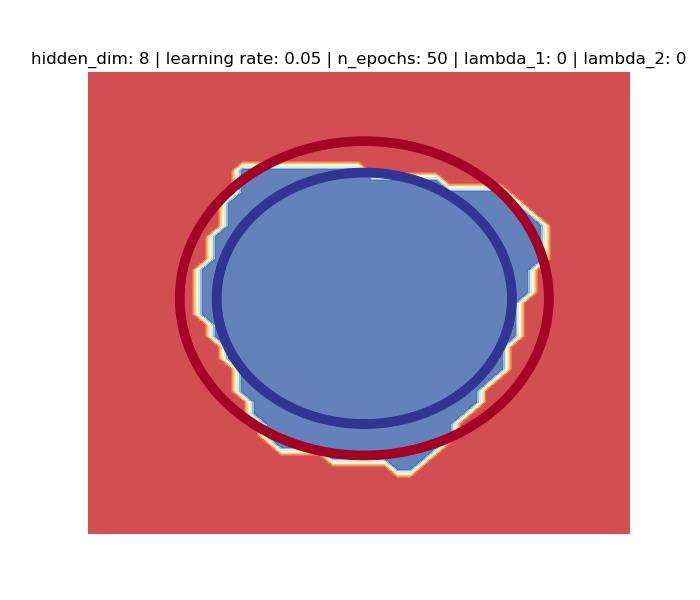
\includegraphics[width=\linewidth]{decision1.jpg}
	\caption{Decision boundary 1}
	\label{fig:boat1}
\end{figure}


\begin{figure}
	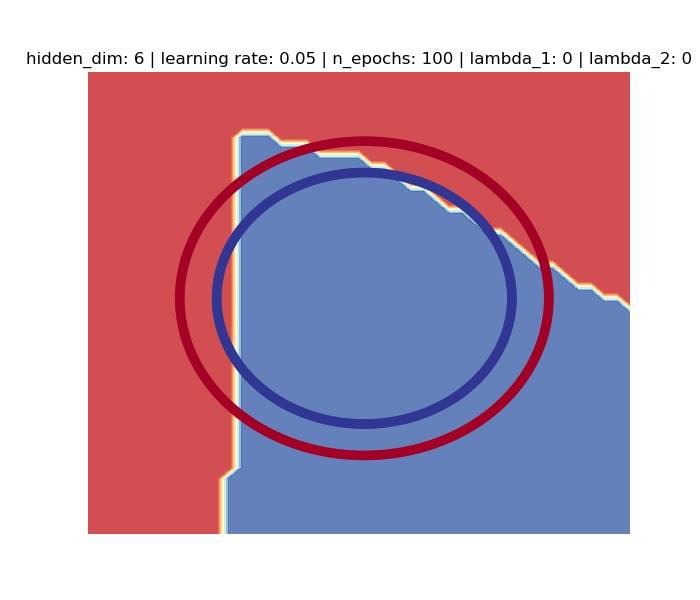
\includegraphics[width=\linewidth]{decision2.jpg}
	\caption{Decision boundary 2}
	\label{fig:boat1}
\end{figure}

\begin{figure}
	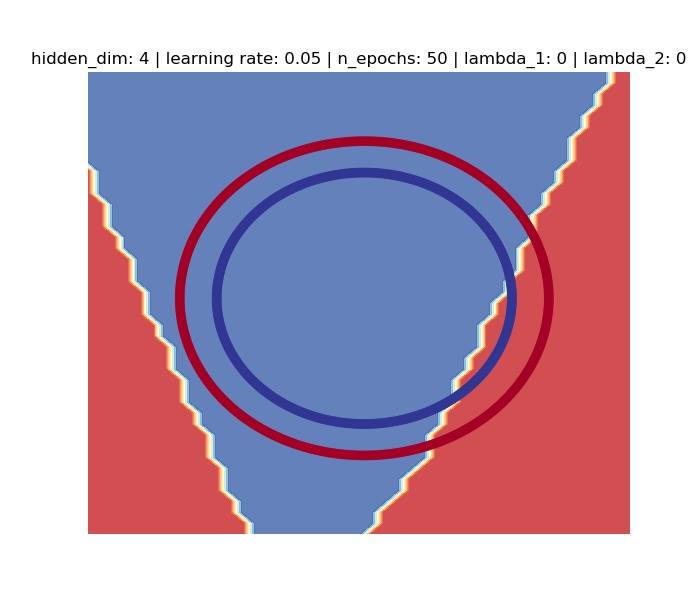
\includegraphics[width=\linewidth]{decision3.jpg}
	\caption{Decision boundary 3}
	\label{fig:boat1}
\end{figure}

\begin{figure}
	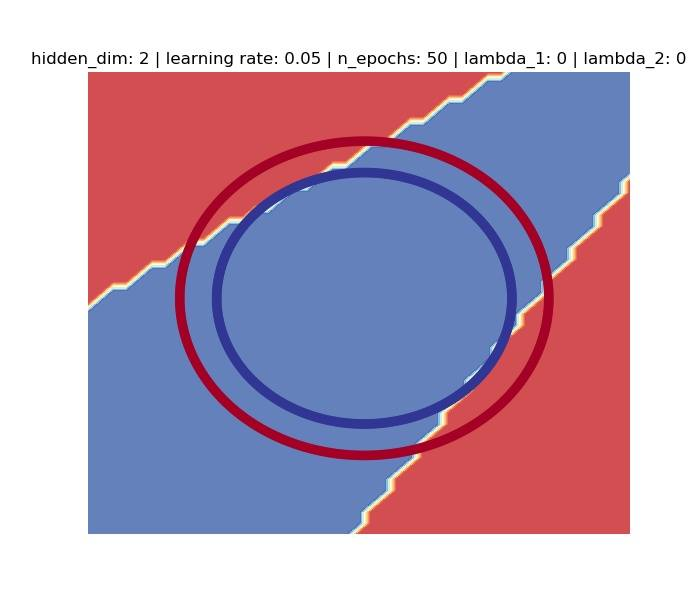
\includegraphics[width=\linewidth]{decision4.jpg}
	\caption{Decision boundary 4}
	\label{fig:boat1}
\end{figure}

\begin{figure}
	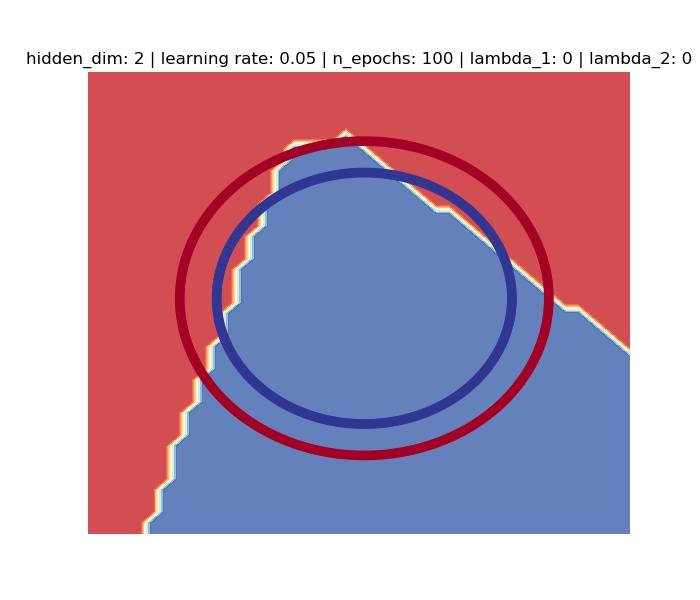
\includegraphics[width=\linewidth]{decision5.jpg}
	\caption{Decision boundary 5}
	\label{fig:boat1}
\end{figure}

\begin{figure}
	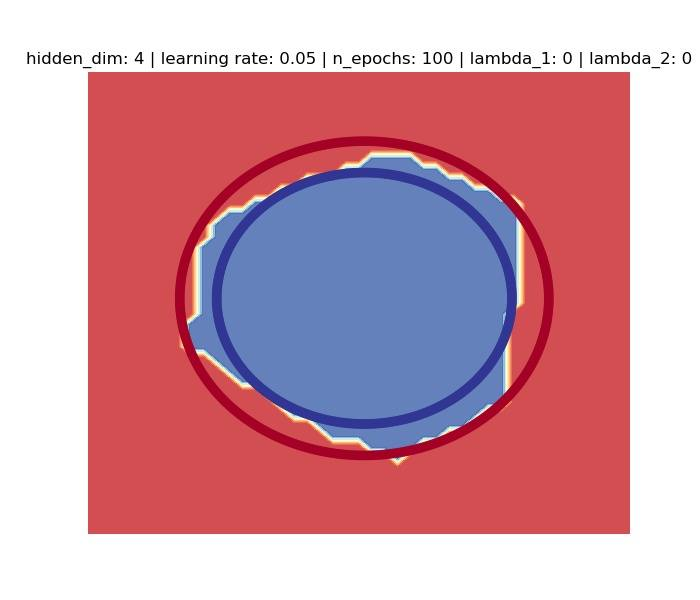
\includegraphics[width=\linewidth]{decision6.jpg}
	\caption{Decision boundary 6}
	\label{fig:boat1}
\end{figure}

\begin{figure}
	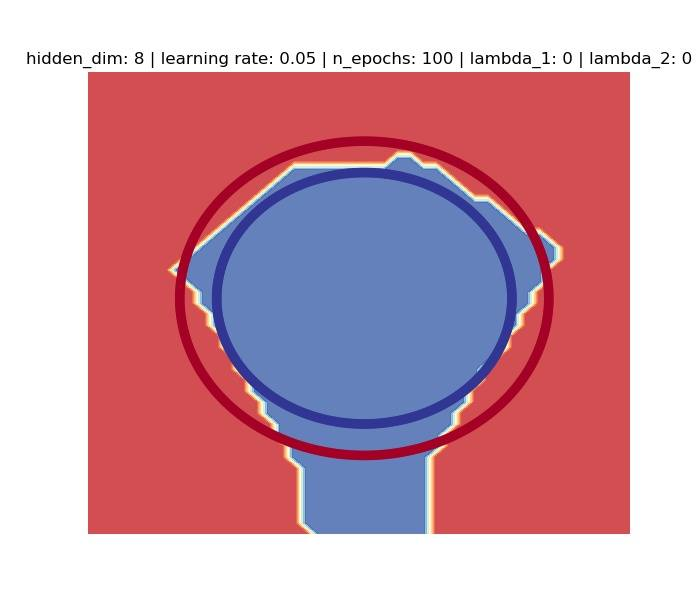
\includegraphics[width=\linewidth]{decision7.jpg}
	\caption{Decision boundary 7}
	\label{fig:boat1}
\end{figure}


\begin{figure}
	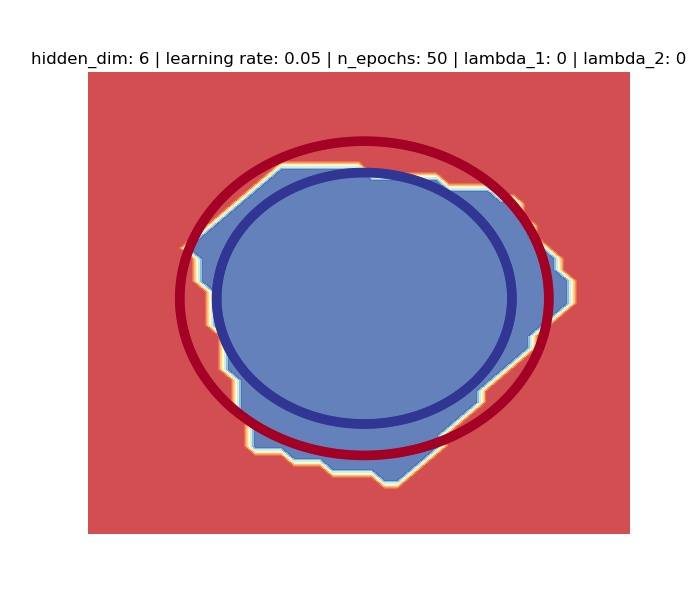
\includegraphics[width=\linewidth]{decision8.jpg}
	\caption{Decision boundary 8}
	\label{fig:boat1}
\end{figure}

\begin{figure}
	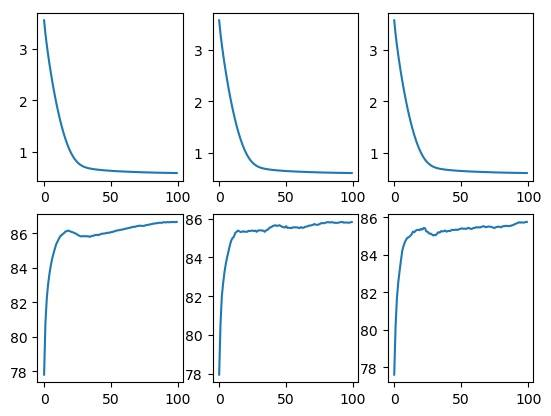
\includegraphics[width=\linewidth]{pic5.jpg}
	\caption{The first row is the loss function plots for each train/valid/test sets, and the second row is the accuracy for each train/valid/test sets. Hyperparamerers: Hidden layer size = 50, learning rate = 0.01, number of epochs = 100, all regularization constant set to 0.001.}
	\label{fig:boat1}
\end{figure}



\end{document}